\section{Experimental Setup}\label{sec:experimentalSetup}

In this section, we describe the setup of our study. First we describe how we mined the data-set of Android app pairs that will serve as a benchmark for our study (Section~\ref{sec:dataset}).  Then, we describe the setup of our infrastructure used to perform the study(Section~\ref{sec:infra}) followed by a discussion on the hardware setup and configurations used (Section~\ref{sec:hardware}). We finally describe the adaptations we performed on the base setup in order to facilitate the individual analyses (Section~\ref{sec:sensitivapi}, \ref{sec:pathsetup}, \ref{sec:manifestAnalysis})

\subsection{Constructing our dataset}\label{sec:dataset} Most malware are simply repackaged versions of benign apps from the official store that injects code performing malicious tasks. Zhou et al.~\cite{DBLP:conf/sp/ZhouJ12} curated a wide-ranging malware collection, where 80\% of samples are know to be built by repackaging benign apps. Because of this our dataset is composed by app pairs (benign-malicious).
\kn{I am not sure how the Zhou's work is the reason we should have app pairs. Did they mention in their study that app pairs are needed. Or is this the basis of our app pairs. Can we simply not justify the need for pairs by saying something in the lines of "We need both versions of a repackaged app to test the accuracy of our tool?"}
%\kn{Here we need one or two lines motivating why we need app pairs.} 

To curate our app pairs, we used Androzoo~\cite{DBLP:conf/msr/AllixBKT16}, a collection of Android apps mined from multiple markets, including the official Google Play~\footnote{\url{https://play.google.com/store}}. Androzoo makes an ideal source of apps as it was designed with a primary goal of aiding research studies such as ours. 

Due to space and time constraints, we capped our download of apps to 20 hours and 42 GB of apps. This resulted in 7268 app pairs. Androzoo sometimes contains multiple malicious versions for the same benign app. In such cases, we picked the first malicious version ensuring that the resulting pairs were unique in terms of their original apps. This step resulted in our dataset containing 1831 app pairs. Among 1831 initial pairs, only 1395 apps could be successfully instrumented by DroidFax. Among the 1395 instrumented pairs, we had installation errors on our emulator (Pixel 4 running Android API 28), many times due to compatibility issues. 

In the end, we obtained 824 valid app pairs that could be used for our study. For time issues, we decided to use just 95 \kn{This number needs to be changed to our final set} pairs at our research. Figure~\ref{fig:stores} presents the markets where the most of malicious version apps were collected according to Androzoo including several from the Google play store.
%\kn{TODO: Convert Table 1 into a bar chart listing only the top 6. The rest of the app stores with less than 10 apps can be listed in the appendix } 


\begin{figure}[ht]
\centering
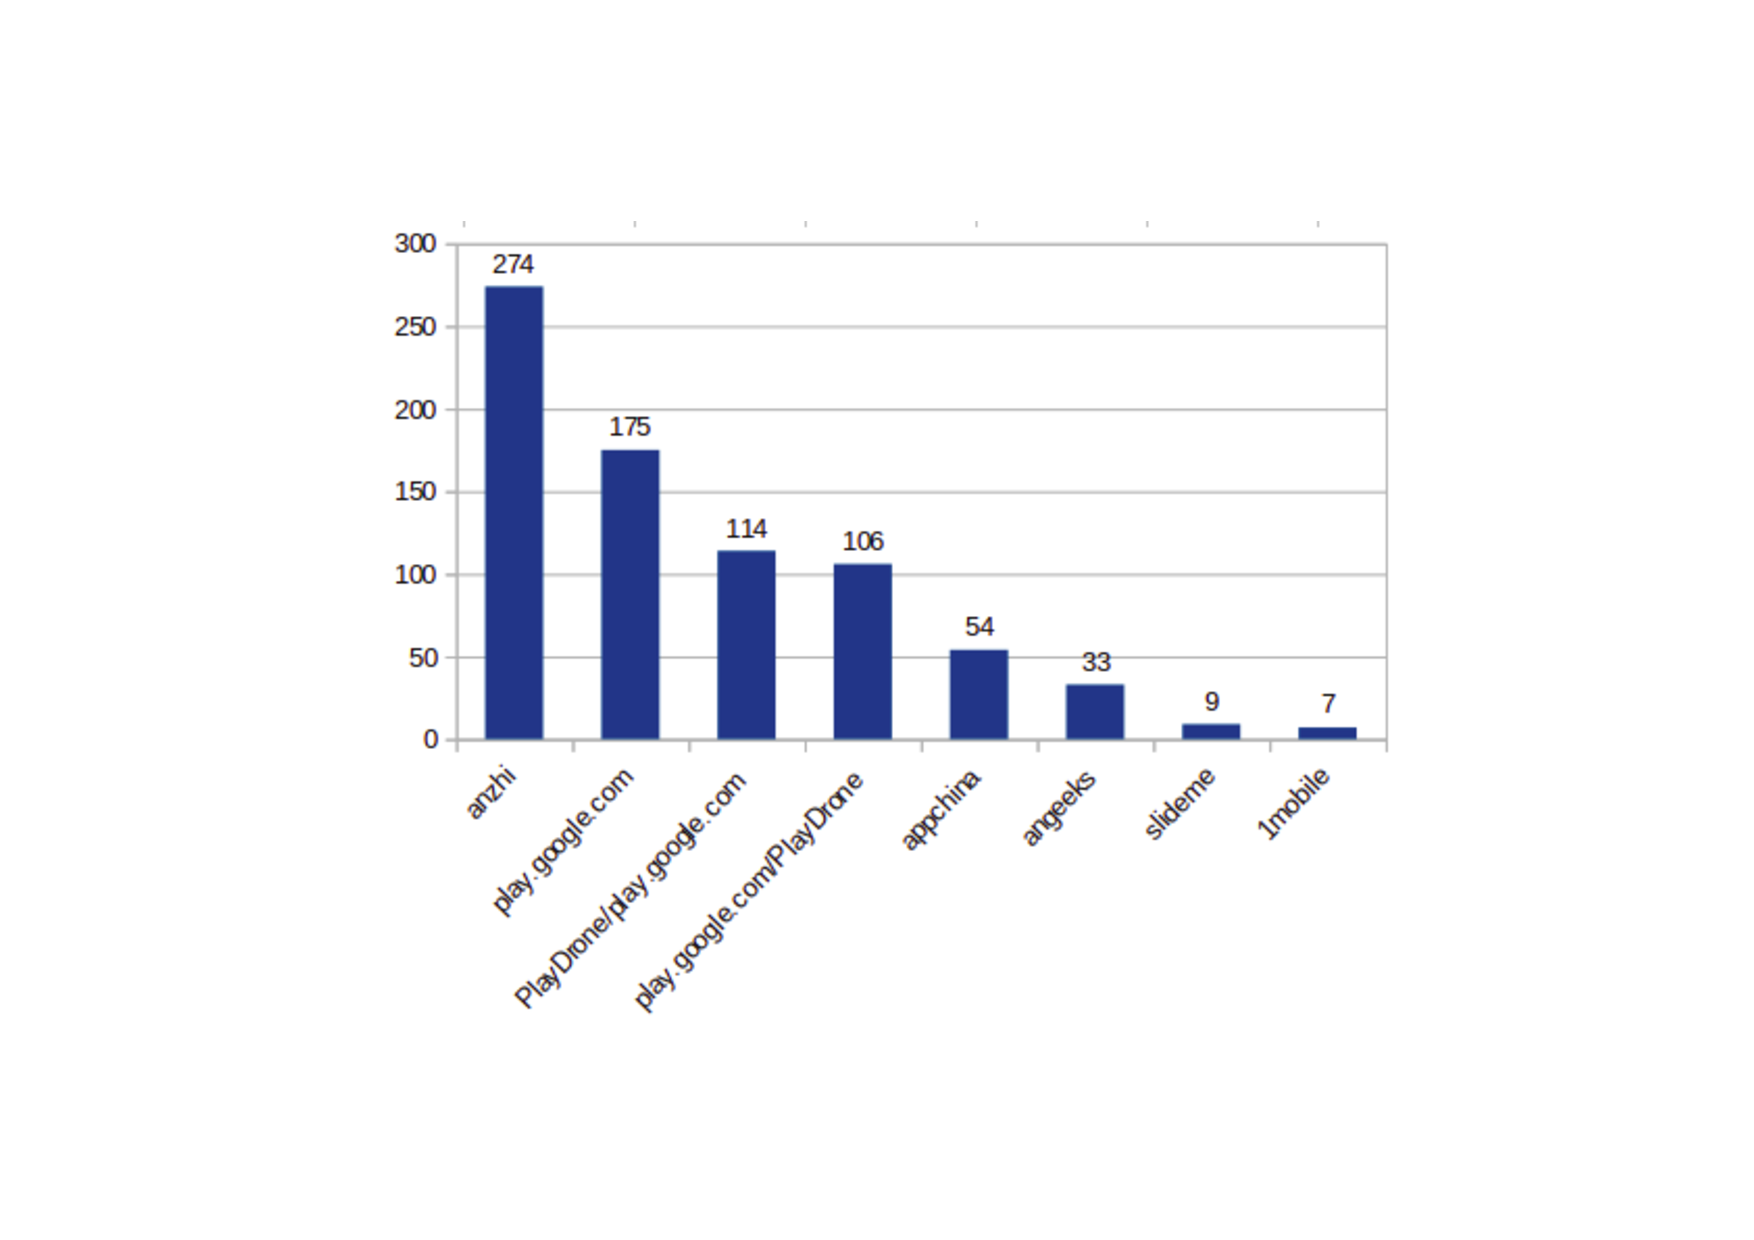
\includegraphics[scale=0.3]{images/stores.pdf}
\caption{Markets where malware was downloaded.}
 \label{fig:stores}
\end{figure}

\kn{I have removed the following as it is inconsistent with our current story. We no longer performn just a study, we offer an approach. And we no longer study all four, only the top one Droidbot and built on top of it. }
In order to understand the limitations in accuracy of mining sandbox approaches, we perform our study and build upon DroidBot~\cite{DBLP:conf/icse/LiYGC17} which is considered as the state of the art in mining sandbox approaches in terms of accuracy. 
%To perform an in-depth analysis of how various factors influence the quality of android sandboxes, we could have used several state of the art test generation tools like: Monkey~\cite{Monkey}, Droidmate2~\cite{DBLP:conf/kbse/BorgesHZ18}, Droidbot~\cite{DBLP:conf/icse/LiYGC17} and Humanoid~\cite{DBLP:conf/kbse/LiY0C19}. However, we considered to use just Droidbot, since several study show that it achieved better performance results when mining sensitives resources in comparison with the state of the art~\cite{DBLP:conf/wcre/BaoLL18,DBLP:journals/jss/CostaMMSSBNR22}. Its applies a depth-first strategy (DFS)~\cite{DBLP:conf/oopsla/AzimN13} to dynamically build GUI models, collecting GUI information and running process information.

\subsection{Infrastructure}\label{sec:infra}

\kn{We currently only use one test generation tool. The following paragraph needs to be adjusted to reflect that} 
For our study, we require an extensive infrastructure that will allow us to integrate different test case generation tools. To this end, we used and extended DroidXP\cite{DBLP:conf/scam/CostaMCMVBC20}, a benchmark tool that allows researchers and developers, to integrate and compare test case generation tools for mining sandboxes.

Using DroidXP, test case generation tools can be integrated and deployed easily~\footnote{The DroidXP benchmark is available at https://github.com/droidxp/benchmark}. Another reason to use DroidXP is that it relies on DROIDFAX~\cite{cai2016understanding}, which allowed us to instruments Android apps and collect important information about their execution. For example, this can be used to query for the calls to the sensitive APIs from an app during executions which is important to monitor malicious behavior. 

%\kn{I have commented out the following and shortened it as this is too verbose information about DroidXP's tooling}
\begin{comment}
The DroidXP relies on a Simple Command Line (CLI) that  provides commands for execution of different experiments with several setup, following parameters:
\newline
\newline
\textbf{DroidXP:} python main.py [-h] [--list-tools] [-tools] toolName [-t] timeSeconds [-r] repetition [--list-outputs] [--output] output [--debug] [--version]\newline
\newline
One can show help message [-h], list available test generation tools [--list-tools], test tools used in the experiment (toolName), threshold of the execution time in the experiment (timeSeconds), number of repetitions used in the experiment (repetition), list available output formats [--list-outputs], output formtat that will be used to show results (default: basic) (output),
run in DEBUG mode (default: false) [--debug] and print DroidXP version [--version].

Follow an example of a command line that executes DroidXP for three minutes (180 seconds), at test generation tools Monkey, repeating all the performance three times, and outputting the final result at a CSV file format:
\newline
\newline
\textbf{python main.py -tools monkey -t 180 -r 3 --output csv}
\newline
\end{comment}


Benchmarking using DroidXP typically happens in three phases:

\textbf{Phase 1: Instrumentation:} In the first phase, a set of APK files is provided as input to DroidXP. This set is composed of all the app pairs (benign/malicious) used in our study. Each APK file is then instrumented to be able to collect data about the execution. This instrumentation is performed using DroidFax. To improve the performance across multiple executions, the set of pairs already instrumented are made available. In this phase, each app is statically analyzed to collect the number of methods and classes inside the app, which is necessary to measure coverage during execution. %\kn{I dont understand this statement, which set are pre-instrumented, whats the instrumentation like, who defines this set}. 

\textbf{Phase 2: Execution:} In this phase, the execution is done by deploying an instrumented APK file in an Android emulator and executing the instrumented app using one or more test generation tools for a chosen period of time. To ensure that each execution gets the benefit of running on a fresh android instance without biases that could stem out of history, all data stored on the emulator from previous executions are wiped out from the emulator. 

%\kn{Is the result analysis into logcat done by DroidXP or an extension by us? In general, it is unclear what is existing in DroidXP already and what we do. Isnt logcat a separate tool. If this is done by DroidXP, please make it clear that DroidXP invokes logcat on its own}%
\textbf{Phase 3: Result Analysis:} During the execution, all the data that is required to compute the results are persisted by DroidXP, using Logcat \cite{Logcat}, one of the Android SDK's native logging tools. This can be used to perform analysis on the results of executing test generators on apps and observe malicious behavior.\newline
\newline
\textbf{DroidXPTrace}. To leverage our study, we also used an auxiliary tool from DroidXP project called DroidXPTrace~\footnote{The DroidXPTrace is also available at https://github.com/droidxp/droidxptrace}. DroidXPTrace allowed us to monitor aspects like dynamic call graphs which was not possible using vanilla version of DroidXP. DroidXPTrace, using the result from Phase 3 of DroidXP, creates a call graph of app pair, exploring traces from its entry point to sensitive API access. In the end, it compares both call graphs (benign and malicious app version), and generated a JSON file recording the following information:
%\kn{I have rephrased the previous paragraph, please check if it is still accurate}. 

%\kn{Overall the following bits in the rest of this subsection are a bit confusing.  You use the word trace and graph interchangeably. is it a graph or a trace. And finally the connection to paths taken comes out of nowhere. I propose rephrasing this part with an example data from some app. Only one of the columns is enough. Even if the example is an artificial one it is fine. Important is that it becomes clear what data is recorded. }
\begin{itemize}
\item \texttt{benign}: Name of log file from the benign app version
\item \texttt{malign}: Name of log file from the malicious app version
\item \texttt{benignGraphs}: call graphs that contain traces with access to sensitive methods in the benign version of the app.
\item \texttt{malignGraphs}: call graphs that contain traces with access to sensitive methods in the malicious version of the app.
\item \texttt{methodsAccessedOnlyByMalign}: The sensitive methods that are accessed only by the malicious version of the app. This information is important to identify if a particular sensitive call that is undetected by a sandbox occurs only in a malicious version.
\item \texttt{benignGraphContainsMalignGraph}: Comparison between benign and malicious sub-callgraphs
\item \texttt{hasDifferentTraces}: whether the benign and malicious app version have different traces to sensitive resources. 
\end{itemize}

 This information helped us to explore traces between an app's entry point and its access to sensitive methods during run time.
 \kn{What I have commented below is talking about the study itself and not the setup. Please ensure other such instances are removed if I have missed them.}
 %This investigation shows that in several situations, although both app versions (benign-malicious) access the same set of sensitive resources, they access them using different traces, which could mean malicious sensitive resource access.

\subsection{Hardware and procedure setup}\label{sec:hardware}

We deployed our experiment on a 32-Core, AMD EPYC 7542 CPU, 512 GB RAM, storage Samsung SSD 970 EVO 1TB machine running a 64-bit Debian  GNU/Linux 11. We also configured our emulator to run all selected apps on Google Android version 9.0, API 28, 512M SD Card, 7GB internal storage, with X86 ABI image.

For our study, we configured DroidXP to run each of the $95$ \kn{This number needs to be changed here too. I suggest introducing a macro for this and using it everywhere to make sure everytime our experiment evolves, we dont need to change this everywhere} app pairs using Droidbot testing tool for three minutes. To mitigate noise, we repeated the full process three times which took in total ($95 \times 2$ apps (benign/malicious) $\times 3$ runs $\times 3$ min) + ($95 \times 2$ apps $\times 1.5$ min for emulator reboot) $\apeq 34$ machine hours.
%\kn{Initial? Was there a follow up study, if not please use only study. This is feedback for all instances with the word initial}

Although it was possible to run more than 10 emulators in parallel on one physical machine, to avoid any interference resulting from context switching within the operating system, we chose to run one emulator at a time. Hence, all evaluation processes took around $3$ days and additional $5$ days for environment deployment.

In the following subsections, we describe the setup required to perform custom analysis that were central to our study.

\subsection{Sensitive API setup} \label{sec:sensitivapi}
\fh{Here the text talk about false positive. We have to change to talk about how we extract the most sensitive APIs used by malicous apps }
\kn{I am ignoring this subsection for review as it is no longer relevant. Please add some details about the sensitive APIs collection so it can be extended upon.}
To perform the false positive analysis we used the infrastructure of DroidXP, described in section~\ref{sec:infra}. After finishing \textbf{Phase 2 (execution)}, we have all explorer information about the apps under analysis by Droidbot test generation tools.

Our analysis concert just at the benign version of apps, since false positive alarm could occur when some expected behavior from the benign app version is not seen during mining step. Hence, as a first step we collect all sensitive methods (SM) by the union of three execution of mine sandbox at all benign apps version. With this step, we could have a base set of sensitive methods called by each benign version from all 95 apps explored in our study. After, we executed mine sandbox again at the same set of benign apps version seven times. At each execution we observed the set of sensitive methods called, and compare them with the initial set of sensitive methods composed by the union of methods explored by the first three executions. In the end, we executed 7 tests, checking if the difference between all the these sets are empty sets, as below:\newline

\begin{enumerate}[(Test 1)]
 \item {$\left\{\left\{SM01\right\} \cup \left\{SM02\right\} \cup \left\{SM03\right\}\right\} \textit{diff} \left\{SM04\right\} = \emptyset$}
 \item {$\left\{\left\{SM01\right\} \cup \left\{SM02\right\} \cup \left\{SM03\right\}\right\} \textit{diff} \left\{SM05\right\} = \emptyset$}
 \item {$\left\{\left\{SM01\right\} \cup \left\{SM02\right\} \cup \left\{SM03\right\}\right\} \textit{diff} \left\{SM06\right\} = \emptyset$}
 \item {$\left\{\left\{SM01\right\} \cup \left\{SM02\right\} \cup \left\{SM03\right\}\right\} \textit{diff} \left\{SM07\right\} = \emptyset$}
 \item {$\left\{\left\{SM01\right\} \cup \left\{SM02\right\} \cup \left\{SM03\right\}\right\} \textit{diff} \left\{SM08\right\} = \emptyset$}
 \item {$\left\{\left\{SM01\right\} \cup \left\{SM02\right\} \cup \left\{SM03\right\}\right\} \textit{diff} \left\{SM09\right\} = \emptyset$}
 \item {$\left\{\left\{SM01\right\} \cup \left\{SM02\right\} \cup \left\{SM03\right\}\right\} \textit{diff} \left\{SM10\right\} = \emptyset$}
 
\end{enumerate}

We observed if all execution explored the same sensitive methods at each benign app in our dataset (95 app pairs). We consider that occur a false positive alert when at least one of seven tests fail, i.e. if one of the 7 tests returns a non-empty set.

As a second step, we also choose a random execution, and check if the set of sensitive methods collected by this execution, is the same of other 9 sensitive methods set, collected by others 9 executions. At this second step, the fifth execution was the choose one as a base execution for tests, as described below:\newline

\begin{enumerate}[(Test 1)] \setcounter{enumi}{7}
 \item {$\left\{SM05\right\} \textit{diff} \left\{SM01\right\} = \emptyset$}
 \item {$\left\{SM05\right\} \textit{diff} \left\{SM02\right\} = \emptyset$}
 \item {$\left\{SM05\right\} \textit{diff} \left\{SM03\right\} = \emptyset$}
 \item {$\left\{SM05\right\} \textit{diff} \left\{SM04\right\} = \emptyset$}
 \item {$\left\{SM05\right\} \textit{diff} \left\{SM06\right\} = \emptyset$}
 \item {$\left\{SM05\right\} \textit{diff} \left\{SM07\right\} = \emptyset$}
 \item {$\left\{SM05\right\} \textit{diff} \left\{SM08\right\} = \emptyset$}
 \item {$\left\{SM05\right\} \textit{diff} \left\{SM09\right\} = \emptyset$}
 \item {$\left\{SM05\right\} \textit{diff} \left\{SM09\right\} = \emptyset$}
\end{enumerate}

As the first analysis, we also consider a false negative occurrence, if one of the 9 remaining tests returns a non-empty set.

\subsection{Trace analysis} \label{sec:pathsetup}

As described at section~\ref{sec:infra}, we take advantage of DroidXP's auxiliary tool, DroidXPTrace to create dynamic call graphs of each app pair (benign/malicious), as executed by Droidbot test generation tool. With these call graphs, we investigated specifically those app pairs that were not described as a malware during the exploratory step, i.e, the test generation tool DroidBot collected the same set of sensitive APIs for both version. If a dynamic call graph of these app pairs presented different traces from entry point to sensitive APIs call at both versions, we suspect this to indicate presence of malware.

Figure~\ref{fig:callGraph} present a example of benign and malicious call graph. Although both app version access the same set of sensitive resources, malicious version follows a different execution trace. 


\begin{figure}[ht]
\centering
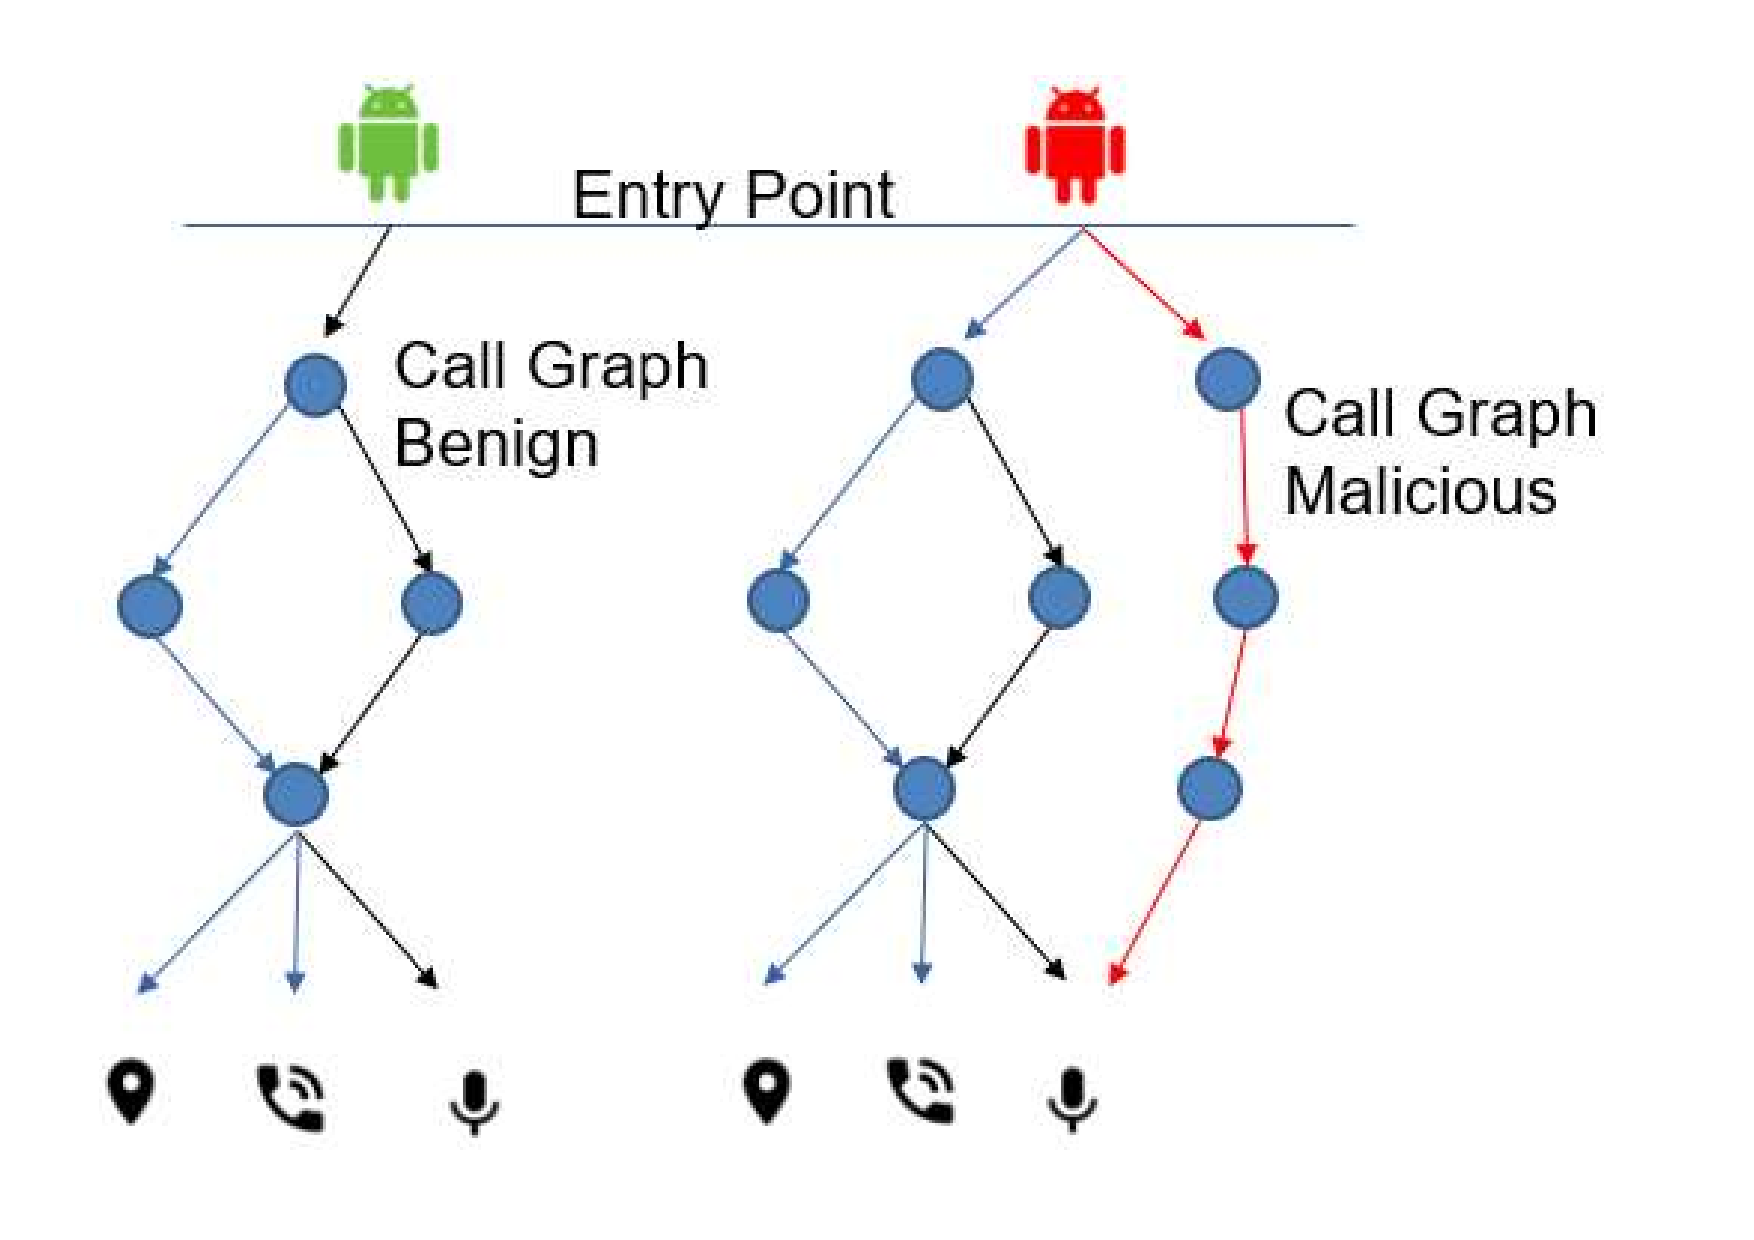
\includegraphics[scale=0.25]{images/maliciousCallGraph.pdf}
\caption{Benign and Malicious call graph.}
 \label{fig:callGraph}
\end{figure}


\subsection{Manifest file analysis}\label{sec:manifestAnalysis}

Our work also observed the Manifest file of all app pairs. These files present essential security information which the Android system must make available before executing an app. Among other things, a  list of requested permissions and a list of important components are persisted in the manifest file. Unfortunately, Manifest files are generally not considered by sandbox approaches when detecting malware inspite of the fact that they can are easily modified by malicious developers~\cite{DBLP:journals/corr/abs-1208-4536}. For instance, by inserting new permission requests or component capabilities (actions). Such injections can happen either manually or through automated scripts.

Automated process sometimes generate Manifest file with duplicate permission requests, as the original app may already contain the permission request. Such duplication also happen when repackaged apps add a component with a capability which was requested by another component. On top of this, our manifest analysis also allowed us to monitor suspicious new permissions or excessive amounts of permissions. 

To extract and analyze the Manifest file, we used an in-house Android SDK analyzer called \textit{apkanalyzer}. We implemented a python script that used \textit{apkanalyzer} and computed which malicious apps had duplicated request permission or duplicated actions. The script also extracted how many permissions were requested by all apps, to help us monitor potential suspicious features. Listing~\ref{lst:androidManifestDupli} and Listing~\ref{lst:androidManifestAction} present an example of duplicated permission extracted from malicious version of the app \textbf{[com.ifeel.frogjump]}, and an example of duplicated component capabilities from malicious version of the app \textbf{[com.koushikdutta.superuser]} respectively:

%\kn{app-8 according to what table? reference please}. 

\begin{lstlisting}[caption={Example of duplicated permission from malicious version of app (com.ifeel.frogjump)}, language=Java,
    basicstyle=\fontsize{6}{5}\selectfont\ttfamily,
    label={lst:androidManifestDupli}]

13:M >  <uses-permission
        android:name="android.permission.READ_PHONE_STATE" />

16:M >  <uses-permission
        android:name="android.permission.ACCESS_COARSE_LOCATION" />

19:M >  <uses-permission
        android:name="android.permission.INTERNET" />

22:M >  <uses-permission
        android:name="android.permission.ACCESS_NETWORK_STATE" />
    .
    .
    .
134:M > <uses-permission
        android:name="android.permission.INTERNET" />

137:M > <uses-permission
        android:name="android.permission.WAKE_LOCK" />

140:M > <uses-permission
        android:name="android.permission.READ_PHONE_STATE" />

143:M > <uses-permission
        android:name="android.permission.ACCESS_NETWORK_STATE" />

146:M > <uses-permission
        android:name="android.permission.WRITE_EXTERNAL_STORAGE" />

149:M > <uses-permission
        android:name="android.permission.ACCESS_WIFI_STATE" />
\end{lstlisting}

\begin{lstlisting}[caption={An example of duplicated component capability from malicious version of app (com.koushikdutta.superuser)}, language=Java,
    basicstyle=\fontsize{6}{5}\selectfont\ttfamily,
    label={lst:androidManifestAction}]

101:M > <receiver
102:M >  android:name=".SuCheckerReceiver">
103:M >  <intent-filter>
104:M >    <action
105:M >      android:name="android.intent.action.BOOT_COMPLETED" />                 
106:M >  </intent-filter>
107:M > </receiver>
108:M > <receiver
109:M >  android:name=".PackageChangeReceiver">
110:M >  <intent-filter>
111:M >    <action
112:M >      android:name="android.intent.action.BOOT_COMPLETED" />
113:M >    <data
114:M >      android:scheme="package" />
115:M > </intent-filter>
     .
     .
     .
\end{lstlisting}

Listing~\ref{lst:androidManifestDupli} suggests that the four first requested permission could have been added automatically. Listing~\ref{lst:androidManifestAction} present a duplicated component where suggests that the first was newly injected by a naive hacking script.